\documentclass[10pt,twocolumn]{article}

\usepackage{amsmath}
\usepackage{amssymb}
\usepackage{amsthm}
\usepackage{appendix}
\usepackage{booktabs}
\usepackage{bm}
\usepackage{graphicx}
\usepackage{multirow}
\usepackage{pifont}
\usepackage{subcaption}
\usepackage{xcolor}

\usepackage[hmargin=.75in, vmargin=1in]{geometry}

\graphicspath{ {./images/} }

\DeclareMathOperator*{\argmin}{argmin}
\DeclareMathOperator*{\minimize}{minimize}
\DeclareMathOperator*{\subto}{subject\,to}

\newcommand{\cmark}{\ding{51}}
\newcommand{\xmark}{\ding{55}}

\begin{document}

\begin{titlepage}
  \begin{center}
    \Huge
    Final Project Report \\
    \hfill \\
    Optimal Control \\ with \\ Nonlinear System Identification

    \vfill

    \Large
    \textbf{Alvin Sun} \\

    \vfill

    Fall 2020 \\
    ECE 551

  \end{center}
\end{titlepage}

\begin{abstract}
  Optimal control, especially for nonlinear systems, has became one of the most powerful
  modern control techniques that produces intelligent behaviors. Most of optimal control
  methods require a-priori knowledge of the system, namely its governing dynamical equations.
  However, in reality, many of the physical systems has unknown or even time-varying dynamics.
  As a result, identifying those dynamics becomes a crucial part in controlling them.
  This project aims at controlling nonlinear plants with unknown dynamics, bringing together
  one of the best performing nonlinear system identification methods, SINDy, with the
  powerful nonlinear model predictive controller.
\end{abstract}

\section{Problem Statement}

The problem of controlling arbitrary systems with unknown dynamics can be divided into
two aspects
\begin{enumerate}
  \item Estimation of the dynamics
  \item Controlling the plant
\end{enumerate}

\subsection{Estimation}

Most of the real-world physical systems can be expressed in the following first order
vector differential equation form
\begin{gather}\label{eqa:fx}
  \dot{x} = f(x)
\end{gather}
where $x$ is the internal states of the system. Despite its simple form, the vector
function $g$ can be arbitrarily complex and nonlinear. To generalize a little more
to fit the settings of control, the dynamical equations becomes
\begin{gather}\label{eqa:fxu}
  \dot{x} = f(x, u)
\end{gather}
where $u$ is a vector for the controlled actuation. Consider the case where the
states are directly observable from the plants, namely, we can obtain both $\dot{x}$
and $x$ from sensor readings, the problem of identifying the system becomes
estimating this nonlinear vector function $f$. For the case where the states
and derivatives are partially observable, we can build a seperate observers and filters dedicated
to estimating the missing variables. For the scope of this project, we assume that everything is
directly obtainable from the plants.

\subsection{Control}
The problem for controlling a dynamical system is fairly simple. The overall objective is
just regulating the states of the system to some desirable location with the help of actuation.
Formally, for all control functions $u(\cdot)$ and initial conditions $x_0$, there
exists a solution to Equation~\ref{eqa:fxu} that can be interpreted as the resulting
state trajectory $x(\cdot)$. We will then have some reference state trajectory
$x_{\mathrm{ref}}(\cdot)$ that we would like the system to achieve. Therefore, the
problem of control is then to find some control function, $u(\cdot)$, such that the
resulting state trajectory is close or even converges to the reference trajectory. However,
due to the limitation of digital computing, we would need to dicretize
Equation~\ref{eqa:fxu} into the following form.
\begin{gather}
  x_{k+1} = F(x_k, u_k)
\end{gather}
Then, instead of finding a function defined in an infinite number of time steps, we only need to
find a finite number of control sequence, $\{u_k\}_{k \in \mathcal{K}}$, which achieves
state tracking on a finite number of state sequences, $\{x_k\}_{k \in \mathcal{K}}$.

\section{Background}

Nonlinear system identification has become a rapidly growing field in the recent years due to
high quality sensors and high performance digital computing becoming more readily available.
There are several approaches that are starting to be widely applied in a variety of applications.
This project has explored two of the popular methods, Koopman Analysis and Sparse
Identification of Nonlinear Dynamics.

\subsection{Koopman Theory}
Koopman Theory is originally proposed in the early 20 century. It stated that any nonlinear
system can be transformed into an infinite dimensional space where the dynamics become
linear. Formally,
\begin{gather}\label{eqa:koopman}
  x_{k+1} = F(x_k) \equiv
  g(x_{k+1}) = \mathcal{K} g(x_k)
\end{gather}
where $g$ is an infinite dimensional nonlinear function and $\mathcal{K}$ is an
infinite dimensional linear operator. Koopman Theory has been brought back to people's
attention in recent years. Dynamic Mode Decomposition \cite{dmd} and its nonlinear
varient eDMD \cite{edmd} are two of the recent system identification approaches that
draw a strong connection to the Koopman Theory. Due to the rapid growth in the development
of neural networks, deep Koopman \cite{deepkoopman} proposed to use an autoencoder network to learn
a finite approximation of the Koopman Operator space of any arbitrary nonlinear system.
However, those work are built around systems without external actuation. \cite{generalkoopman}
generalizes Koopman Theory to systems with control inputs with
\begin{gather}\label{eqa:koopman_ctrl}
  g(x_{k+1}, u_{k+1}) = \mathcal{K}g(x_k, u_k)
\end{gather}
which also drew a strong connection to \cite{dmdc}, which incorporate control inputs with the
DMD method. The major attraction on Koopman related approaches centers around the ability
to linearize a nonlinear system in a global sense. Many of those work focuses on the estimation
aspects of identifying an unknown nonlinear plant, but The connection between classical
linear control theory and Koopman analysis has yet to be explored.

\subsection{Sparse Identification}
Another type of methodology is built around explicitly recovering the structure of
the dynamical equations. A recent framework, SINDy \cite{sindy} (Sparse Identification of
Nonlinear Dynamics), is developed to estimate
for both the structure and coefficients of the nonlinearity of a dynamical system.
They put the Equation~\ref{eqa:fx} into the form
\begin{gather}\label{eqa:sindy}
  \dot{x} = \theta(x) A
\end{gather}
where $\theta$ is a nonlinear vector function that transforms the states with
some predefined nonlinearity such as sinusoids and polynomials, and $A$ is a sparse
coefficient matrix corresponding to each of those nonlinear terms. The popularity
of SINDy based approaches grew rapidly due to its simplicity. SINDYc \cite{sindyc} further
generalizes SINDy to incorporate external control inputs, modeling Equation~\ref{eqa:fxu}
in similar fashion.
\begin{gather}\label{eqa:sindyc}
  \dot{x} = \theta(x, u) A
\end{gather}
Similar to Deep Koopman, autoencoder-like neural network is also applied in \cite{deepsindy}
to learn a latent space coordinate capable of compressing high dimensional measurement
data. Because of the simplicity, the SINDy family methods can also be potentially applied
in an online adaptive setting.

\subsection{Model Predictive Control}

Linear systems are very well studied and have closed-form solutions and properties
for many control scenarios. For example, Linear Quadratic Regulator, which is a form of
optimal controller on linear systems, has closed form solutions for both finite horizon
and infinite horizon cases. Those solutions are known as Riccati Differential Equations
and Algebraic Riccati Equation. For nonlinear systems, however, they are much harder to
control in general. There are many advanced
theories established around stablizing those systems, but for this project, we will
focus on applying model predictive controller directly to obtain actuated nonlinear
behaviors. Model Predictive Control (MPC) is considered the de facto optimal control
technique that is widely applied to a variety of industries nowadays. It can be combined
with system identification techniques to control systems with unknown dynamics. MPC formulates
control objectives as a constrained optimization problem. As a result, the optimal solution
inheritly explores the nonlinear state space which results in intelligent control behaviors.

\section{Methodologies}

There are three main components to this project:
\begin{enumerate}
  \item Synthetic data generation from simulated dynamical systems
  \item Nonlinear system identification
  \item Nonlinear optimal control
\end{enumerate}

\subsection{Simulation}\label{sec:sim}

I chose three systems to verify the effectiveness of my design in combining
system identification with optimal control. Each of them has a nonlinear governing equation
\begin{enumerate}
  \item Simple Rod Pendulum.
    \begin{gather}\label{eqa:pendulum}
      I \ddot{\theta} = -mgl \sin{\theta} - b\dot{\theta} + \tau
    \end{gather}

  \item Lorenz Attractor
    \begin{gather}\label{eqa:lorenz}
      \left\{\begin{aligned}
        \dot{x} &= \sigma (y - x) + u \\
        \dot{y} &=x (\rho - z) - y \\
        \dot{z} &=xy - \beta z
      \end{aligned}\right.
    \end{gather}

  \item Planar Rotor
    \begin{gather}\label{eqa:rotor}
      \left\{\begin{aligned}
        m\ddot{x} &= -(u_l + u_r) \sin{\theta} \\
        m\ddot{y} &= (u_l + u_r) \cos{\theta} - mg \\
        I\ddot{\theta} &= r(u_r - u_l)
      \end{aligned}\right.
    \end{gather}
\end{enumerate}
Using the ground truth model, I can obtain a time series of state evolutions for
each of the chosen systems by applying some white noise control intputs. Since
this project focuses on the effectiveness of the overall system for controlling
nonlinear plants with unknown dynamics, we assume all the states as well as derivatives
are directly observable. To make the simulation more realistic, various level of white noises
are added to the observations. The generated synthetic data is then passed down to
the system identification algorithms.

\subsection{System Identification}

For this project, I originally proposed to build on top of the Deep Koopman work and to
explore its relationship with linear control theories. However, the qualities of system
identification was not good enough to apply control algorithms. As a result, I steered
my project towards the SINDy based system identification methods, and combined that
with nonlinear MPC to achieve the control objectives. In this section, I will discuss
both SINDy and Koopman based methods that I pursued regardless of their success or failure.

\subsubsection{Deep Koopman with Control}\label{sec:deep_koopman}

The original Deep Koopman \cite{deepkoopman} learns the $g$ function in
Equation~\ref{eqa:koopman}, for dynamical systems without external control inputs.
I extended their ideas to incorporate control variables as well as for continuous cases.
Generally, we would like learn some nonlinear transformations
\begin{gather}
  z = \varphi_z(x, u) \\
  v = \varphi_v(x, u)
\end{gather}
such that we have a linear dynamics on those latent space
\begin{gather}
  \dot{z} = Az + Bv
\end{gather}
for some matrix $A$ and $B$. For the purpose of proving of concept, we consider
the special case where $u$ enters the dynamics additively.
With this assumption, we could decouple the nonlinear transformations on the states and
control inputs. Namely,
\begin{gather}
  z = \varphi_z(x) \\
  v = \varphi_v(u)
\end{gather}
An overview of the network architecture is shown in Figure~\ref{fig:koopman_arch}. In
addition to training the autoencoder that should reconstruct the original states and inputs
as accurate as possible, we also want the network to learn a Koopman invariant subspace
that is capable of computing the dynamics with linear equations. Therefore, it is necessary
to obtain ground truth $\dot{z}$ from the training data. Applying the chain rule in
calculus, we obtain
\begin{equation}
  \begin{aligned}
    \dot{z} &= \frac{d}{dt} \varphi_x(x) \\
            &= \nabla \varphi_x(x) \cdot \frac{dx}{dt} \\
            &= \nabla \varphi_x(x) \cdot \dot{x}
  \end{aligned}
\end{equation}
With the help of modern deep learning framework such as TensorFlow, $\nabla \varphi(x)$ can
be easily obtained from automatic differentiation. Now we can construct the different losses
for training the network.
\begin{enumerate}
  \item Autoencoder reconstruction loss for states
    \begin{gather}
      \mathcal{L}_x = \| x - \tilde{\varphi}_x^{-1}(\varphi_x(x)) \|^2
    \end{gather}

  \item Autoencoder reconstruction loss for control inputs
    \begin{gather}
      \mathcal{L}_u = \| u - \tilde{\varphi}_u^{-1}(\varphi_u(u)) \|^2
    \end{gather}

  \item Koopman space linear dynamics loss
    \begin{gather}
      \mathcal{L}_{\mathcal{K}} = \| \nabla \varphi_x(x) \dot{x} -
                                     (A\varphi_x(x) + B\varphi_u(u) ) \|^2
    \end{gather}
\end{enumerate}
The final loss is a weighted summation of the three terms. We can then jointly train the
weights of the neural network and the lineary dynamics matrices $A$ and $B$.

\subsubsection{SINDy with Control \cite{sindyc}}
In order to recover the structure of Equation~\ref{eqa:fxu} for arbitrary sytsem,
SINDYc method assumes the governing equation to be in the form of a summation of
multiple nonlinear terms. For example, the Lorenz Attractor as modeled by
Equation~\ref{eqa:lorenz} can be rewritten in the form of Equation~\ref{eqa:sindyc}.
\begin{gather}\label{eqa:lorenz_sindy}
  \underbrace{
    \begin{bmatrix}
      \dot{x} & \dot{y} & \dot{z}
    \end{bmatrix}
  }_{\dot{x}}
  =
  \underbrace{
    \begin{bmatrix}
      x & y & z & u & xy & xz
    \end{bmatrix}
  }_{\theta(x, u)}
  \underbrace{
    \begin{bmatrix}
      {\color{orange}-\sigma} & {\color{blue}\rho} & 0 \\
      {\color{orange}\sigma} & {\color{blue}-1} & 0 \\
      0 & 0 & {\color{violet}-\beta} \\
      {\color{orange}1} & 0 & 0 \\
      0 & 0 & {\color{violet}1} \\
      0 & {\color{blue}-1} & 0
    \end{bmatrix}
  }_{A}
\end{gather}
With the synthetic dynamical data, we are able to obtain a time series of measurements
on both the states and the derivatives. We can construct the nonlinear dictionary
$\theta(\cdot, \cdot)$ with some commonly seen nonlinearity such as polynomials and
sinusoids. The problems for estimating the dynamical equation then reduces to a
linear regression problem.
\begin{gather}
  \begin{aligned}
    A &=  \argmin_A \| \bm{\theta}(\bm{x}, \bm{u})A - \dot{\bm{x}} \|^2 \\
      &= (\bm{\theta}^T \bm{\theta})^{-1}\bm{\theta}^T \dot{\bm{x}}
  \end{aligned}
\end{gather}
However, in reality, the measured data is noisy, and doing the direct linear regression
will result in a dense coefficient matrix $A$. To solve for this problem, we follow
the Sequential Thresholded Least Square algorithm as mentioned in SINDy \cite{sindy}.
Instead, we solve for a ridge linear regression, which penalizes the magnitude of the coefficients
with their $\mathcal{L}_2$ norm.
\begin{gather}\label{eqa:ridge_regression}
  \begin{aligned}
    A &= \argmin_A \| \bm{\theta}(\bm{x}, \bm{u})A - \dot{\bm{x}} \|^2 + \lambda \| A \|^2 \\
      &= (\bm{\theta}^T \bm{\theta} + \lambda I)^{-1}\bm{\theta}^T \dot{\bm{x}}
  \end{aligned}
\end{gather}
We can drop out terms in $A$ that are below some threshold, and iteratively perform the
ridge linear regression on a subsets of dimensions, until the number of nonzero coefficients
converges. This will help obtain a parsimonious model that not only accurately estimates the
dynamics, but also correctly recovers the underlying structure of the governing equation.

\subsection{Finite Horizon MPC}\label{sec:mpc}

This project uses the direct transcription method, which explicitly formulate the finite horizon
MPC as a constrained optimization problem. Consider the following discrete dynamics,
\begin{gather}
  x_{k+1} = F(x_k, u_k)
\end{gather}
we can define a finite window $h$ such that the MPC can optimize for the future $h$-step
control inputs. Namely, the cost at step $k$ be generally formulated as
\begin{gather}
  J = m(x_h) + \sum_{i=1}^h l(x_i, u_{i-1})
\end{gather}
where $h(\cdot, \cdot)$ imposes some per-step penalties on both the states and the control inputs
and $m(\cdot)$ imposes some penalty on the final state of the future window. For the purpose
of this project, I simplified the cost by removing the $m$ function and
by applying quadratic costs for both control inputs and states.
\begin{gather}
  J = \sum_{i=1}^h x_i^T Q x_i + u_{i-1}^T R u_{i-1}
\end{gather}
for some positive definite matrices $Q$ and $R$. To decouple the effects between different
states and inputs, the matrices can be further simplified to be diagonal. The diagonal entires
then can be interpreted as a trade off on how much we want to regulate each state and each
inputs. The MPC controller can then be formulated as jointly optimizing for the states and
control inputs subject to the dynamics constraints. Namely,
\begin{gather}
  \begin{aligned}
    \minimize_{\begin{subarray}{c}u_0,\ldots,u_{h-1} \\ x_1,\ldots,x_h\end{subarray}}\quad &J \\
      \subto\quad &x_{k+1} = F(x_k, u_k),\; k=0,\ldots,h-1 \\
      &\text{additional constraints}
  \end{aligned}
\end{gather}
This problem can be solved using \texttt{Scipy Optimization Toolbox}.
The system identification, however, gives continuous time dynamics. Therefore, we need to discretize
it in order to make use of finite dimensional optimization tools described above.
We first notice the integral form as following.
\begin{gather}
  x(t + \Delta t) = x(t) + \int_t^{t + \Delta t} f(x(\tau), u(\tau)) d\tau
\end{gather}
If we use small enough time step, and approximate the integral with forward Euler integration,
we can write the dynamics in a discrete fashion.
\begin{gather}
  x_{k+1} \approx x_k + f(x_k, u_k) \Delta t = F(x_k, u_k)
\end{gather}
However, in order to make Euler integration to be accurate, the time step often time needs to be
on the order of $10^{-3}$ second. On the other hand, the finite window is usually around 5 seconds.
This introduces way too many variables for the optimization problem. This problem can be
mitigated by reusing the same control inputs to perform multiple integration steps. For example
we can keep a integration step of $10^{-3}$ second, but performing a dynamical prediction
every 100 integrations. Effectively, we will achieve a prediction step of $0.1$ second. This
method still maintain the discrete dynamics structure, $k_{k+1} = f(x_k, u_k)$, while making
the optimization tractable by reducing the number of free variables.

\section{Results}

In this section, I will first analyze the failure of my originally proposed Deep Koopman with
Control method, and then I will analyze performance for SINDYc method
on all three nonlinear dynamical systems described in Section~\ref{sec:sim}. I will also discuss
the control performance on those systems with the identified model with the SINDYc framework.

\subsection{System ID with Koopman}

An experiment is conducted to learn a single pendulum dynamics using the method proposed
in Section~\ref{sec:deep_koopman}. The neural network is constructed with 2 hidden layers
for both encoders and decoders, where there are 80 hidden neurons at each layers. The
latent space for the states has 16 dimensions and 2 dimensions for controls, i.e.
$z \in \mathbb{R}^{16}$ and $v \in \mathbb{R}^2$. The validation settings for the pendulum
is using a random intial condition with a sinusoidal input. Figure~\ref{fig:koopman_predict}
shows a qualitative results of using the learned Koopman space to perform linear dynamics update
with a given initial condition. When comparing with the ground truth in this one-second window,
it is clear that the
Koopman space prediction does not capture the nonlinear behaviors well. In fact, the prediction
diverges quickly from the ground truth. We can also see the training still has some effects
on forcing the linear prediction to have locally accurate prediction.
Figure~\ref{fig:koopman_correct} shows another comparison where the prediction is manually
brought back to the ground truth every 50 ms. Still, the model prediction is not accurate enough
to perform any nonlinear control behaviors.

\subsection{System ID with SINDYc}

\begin{table*}[htb!]
  \centering

  \begin{tabular}{@{}llclclc@{}}
    \toprule
    \multirow{3.5}{*}{\shortstack{Noise \\ Level}} &
      \multicolumn{2}{c}{Pendulum} &
      \multicolumn{2}{c}{Lorenz Attractor} &
      \multicolumn{2}{c}{Planar Rotor} \\
    \cmidrule(l{3pt}r{3pt}){2-3} \cmidrule(l{3pt}r{3pt}){4-5} \cmidrule(l{3pt}r{3pt}){6-7}
    {} & Validation & Structure & Validation & Structure & Validation & Structure \\
    {} & MSE & Recovered & MSE & Recovered & MSE & Recovered \\

    \midrule

    1e-3 & 2.42e-7 & \cmark & 8.34e-7 & \cmark & 2.32e-6 & \cmark \\
    5e-3 & 4.80e-6 & \cmark & 3.44e-6 & \cmark & 3.09e-6 & \cmark \\
    1e-2 & 2.26e-4 & \cmark & 7.03e-5 & \cmark & 4.03e-6 & \cmark \\
    5e-2 & 5.33e-3 & \xmark & 3.28e-4 & \cmark & 1.44e-5 & \cmark \\
    1e-1 & -       & -      & 2.23e-3 & \cmark & 1.41e-3 & \xmark \\

    \bottomrule
  \end{tabular}

  \caption{SINDYc Performance}
  \label{tbl:sindyc}
\end{table*}

Using the SINDYc framework with Sequential Thresholded Least Square solver, I am able to obtain
very accurate model despite the presence of noise in the training data. Table~\ref{tbl:sindyc}
shows the system identification performance on all of three systems:
\begin{itemize}
  \item The noise standard deviation is represented with the multiple of the
    standard deviation of the original dataset variation.
  \item Validation MSE calculates a metric on how good the estimated model behave
    on validation dataset.
  \item The algorithm is said to successfully recover the structure of the dynamics if
    it identifies the correct nonzero terms in the sparse matrix.
\end{itemize}
Hyperparameter settings for each of the systems are attached in the
Appendix Section~\ref{sec:hyper_sindy}.

\subsection{MPC with SINDYc}

With the identified systems, now we can control those plants with the nonlinear MPC as
described in Section~\ref{sec:mpc}. For each of systems, I used the regression model coming
from the dataset generated with noise level 1e-2. This way, we get a descent amount of
noise while ensuring correct model structure recovery. Animated results are contained
in the notebooks from the source code.

\subsubsection{Pendulum}

The ground truth model parameters in Equation~\ref{eqa:pendulum}
are specified in Table~\ref{tbl:pendulum_params}.
\begin{table}[h]
  \centering
  \begin{tabular}{cccc}
    \toprule
    $m$ [kg] & $l$ [m] & $b$ [N$\cdot$m / (rad/s)] & $I$ [kg$\cdot$m$^2$] \\
    \midrule
    1 & 2/5 & 1/10 & 4/25 \\
    \bottomrule
  \end{tabular}
  \caption{Pendulum Model Parameters}
  \label{tbl:pendulum_params}
\end{table}
An absolute torque saturation of 1.2 N$\cdot$m is also applied to the MPC constraints.
Figure~\ref{fig:mpc_pendulum} shows that under such extreme saturation, the optimization
is capable of coming up with swing up / down controller to perform accurate reference tracking.

\subsubsection{Lorenz Attractor}

The ground truth model parameters in Equation~\ref{eqa:lorenz} are specified in
Table~\ref{tbl:lorenz_params}.
\begin{table}[h]
  \centering
  \begin{tabular}{ccc}
    \toprule
    $\sigma$ & $\rho$ & $\beta$ \\
    \midrule
    10 & 28 & 8/3 \\
    \bottomrule
  \end{tabular}
  \caption{Lorenz Attractor Parameters}
  \label{tbl:lorenz_params}
\end{table}
This system is particularly more difficult for both identification and control. A slightest
bit of error will cause the prediction to diverge exponentially due to its chaotic nature.
More interestingly, this system is underactuated. It has 3 degrees of freedom while having
only one actuator. Nevertheless, Figure~\ref{fig:mpc_lorenz} demonstrated that the system
is still capable of performing good reference trakcing in such challenging chaotic scenario.

\subsubsection{Planar Rotor}

The ground truth model parameters in Equation~\ref{eqa:rotor} are specified in
Table~\ref{tbl:rotor_params}.
\begin{table}[h]
  \centering
  \begin{tabular}{ccc}
    \toprule
    $m$ [kg] & $l$ [m] & $I$ [kg$\cdot$m$^2$] \\
    \midrule
    2 & 1/2 & 1/24 \\
    \bottomrule
  \end{tabular}
  \caption{Planar Rotor Parameters}
  \label{tbl:rotor_params}
\end{table}
This experiment specified the rotor to fly between two waypoints while performing a
flip for each waypoint transition. With an accurately identified model, the nonlinear MPC
algorithm is able to explore the highly nonlinear state space to perform such maneuver.
Figure~\ref{fig:mpc_rotor} shows both the rotation tracking and position tracking of the rotor,
and we can see the flip behavior is done by accurately tracking the rotation reference.

\section{Discussion}

For the failure of learning a good linear embedding for a nonlinear pendulum system, there
are several explanations that could back up this experiental results. By Koopman Theory, it is
known that not all systems can be trasformed into a finite dimensional Koopman Invariant subspace.
On the Control Theory side, we also know that linear systems only have one fixed point at
the origin, so it cannot really represent any systems with multiple fixed points. Even though
the single pendulum is one of the simplest nonlinear systems, its phase plane exhibits an
orbital behavior with infinite numbers of fixed points. Both of these theories explain why it
is very hard to obtain a finite dimensional approximation of that infinite dimensional space
where the Koopman Operator lives in. There is, I believe, another direction to pursue.
We can relate more closely to the general forms of Koopman Analysis with Control given by
\cite{generalkoopman}. Instead of seperately learning the embeddings for states and control
inputs, we can jointly perform the estimation. However, this will also requires additional
thoughts to be connected to linear control theories as it changes the formulations.\\

On the other side, this project successfully demonstrated
the capabilities of combining SINDYc system identification method with nonlinear
Model Predictive Control. It is really fascinating to see how we could create intelligent control
behaviors on highly nonlinear systems with unknown dynamics. A future direction is to make
the system identification run online in an adaptive fashion. This could also potentially deal
with time varying dynamics in the system. Another interesting direction is to come up
with control strategies that provide more information to the estimation process when
we don't have a reliable model. This can potentially reduce the amount of data needed to
identify an accurate and parsimonious model. One challenge of the SINDYc method is that
it does not perform well with implicit dynamics such as double pendulums or acrobots.
Equivalently, those implicit dynamics introduces many fractional nonlinearities that
are really hard to model as nonlinear libraries. Some work, such as \cite{implicitsindy},
has been done to tackle this difficulty, but it remains a big challenge for SINDy based
nonlinear identification methods.

% citations
\newpage
\bibliography{citations}
\bibliographystyle{ieeetr}

% appendix
\newpage
\onecolumn
\appendix
\appendixpage

\section{Source Code}

\section{SINDYc Settings}\label{sec:hyper_sindy}

All hyperparameters for applying the SINDYc algorithm are included
in the \texttt{<model>\_params.py} files in the source code. Table~\ref{tbl:sindyc_params}
shows a summary of those parameters. $\lambda$ is the $\mathcal{L}_2$ regularization
defined in Equation~\ref{eqa:ridge_regression}. The thresholds are used in the
Sequential Thresholded Least Square algorithm to drop out small coefficients at the end of
each iteration.

\begin{table}[h]
  \centering
  \begin{tabular}{llcc}
    \toprule
    Model & Nonlinear Library & $\lambda$ & Threshold \\
    \midrule

    \multirow{2}{*}{Pendulum} & Identity & \multirow{2}{*}{8} & \multirow{2}{*}{0.1} \\
    {} & Sinusoids \\
    \cmidrule{2-4}

    Lorenz Attractor & Polynomial (deg. 2) & 1 & 0.1 \\
    \cmidrule{2-4}

    \multirow{4}{*}{Planar Rotor} & Identity & \multirow{4}{*}{20} & \multirow{4}{*}{0.1} \\
    {} & Sinusoids \\
    {} & Multiplication \\
    {} & Constant \\
    \bottomrule
  \end{tabular}
  \caption{SINDYc Hyperparameters}
  \label{tbl:sindyc_params}
\end{table}

\section{Figures}

\begin{figure}[htb!]
  \centering
  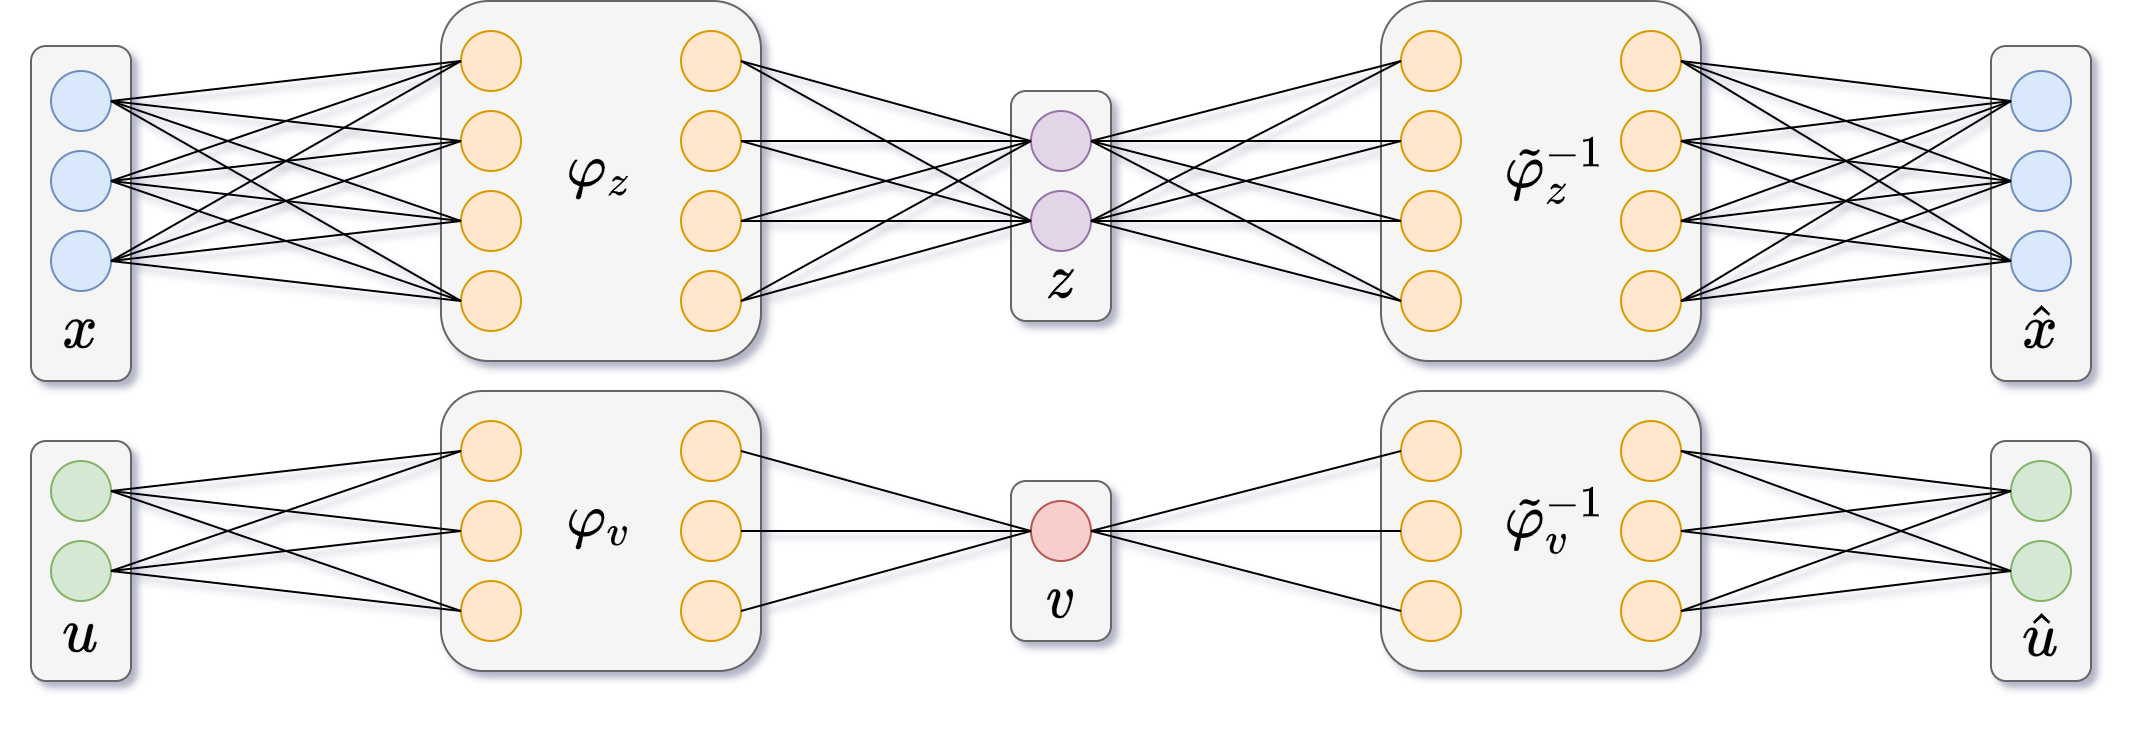
\includegraphics[width=.9\textwidth]{koopman_arch}
  \caption{Deep Koopman with Control}
  \label{fig:koopman_arch}
\end{figure}

\begin{figure}[htb!]
  \centering
  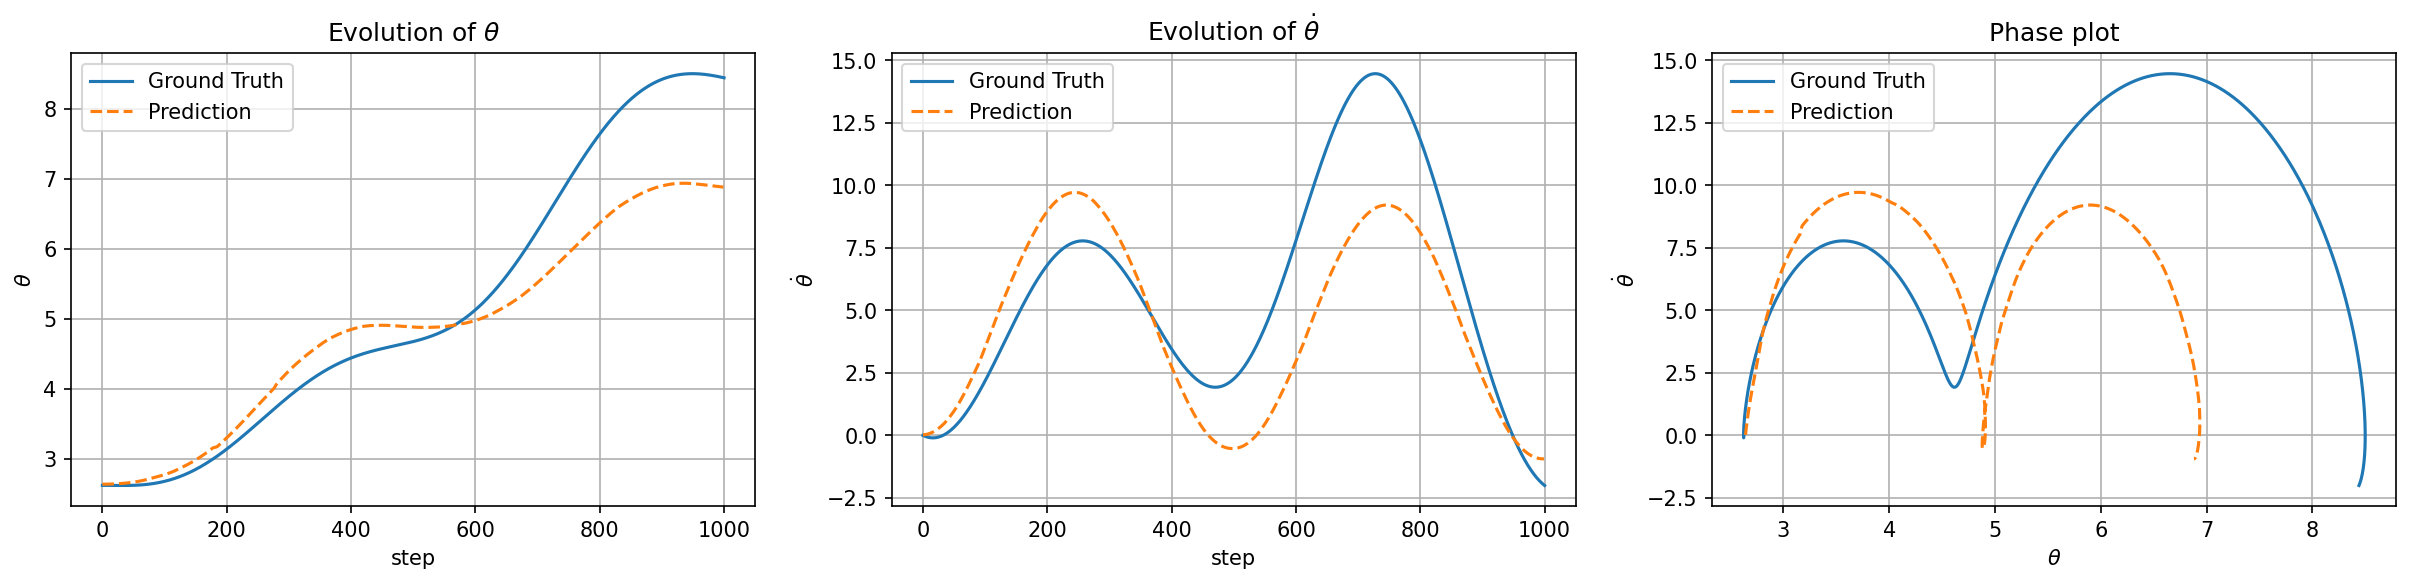
\includegraphics[width=\textwidth]{koopman_predict}
  \caption{Identified Pendulum with Koopman Space Prediction}
  \label{fig:koopman_predict}
\end{figure}

\begin{figure}[htb!]
  \centering
  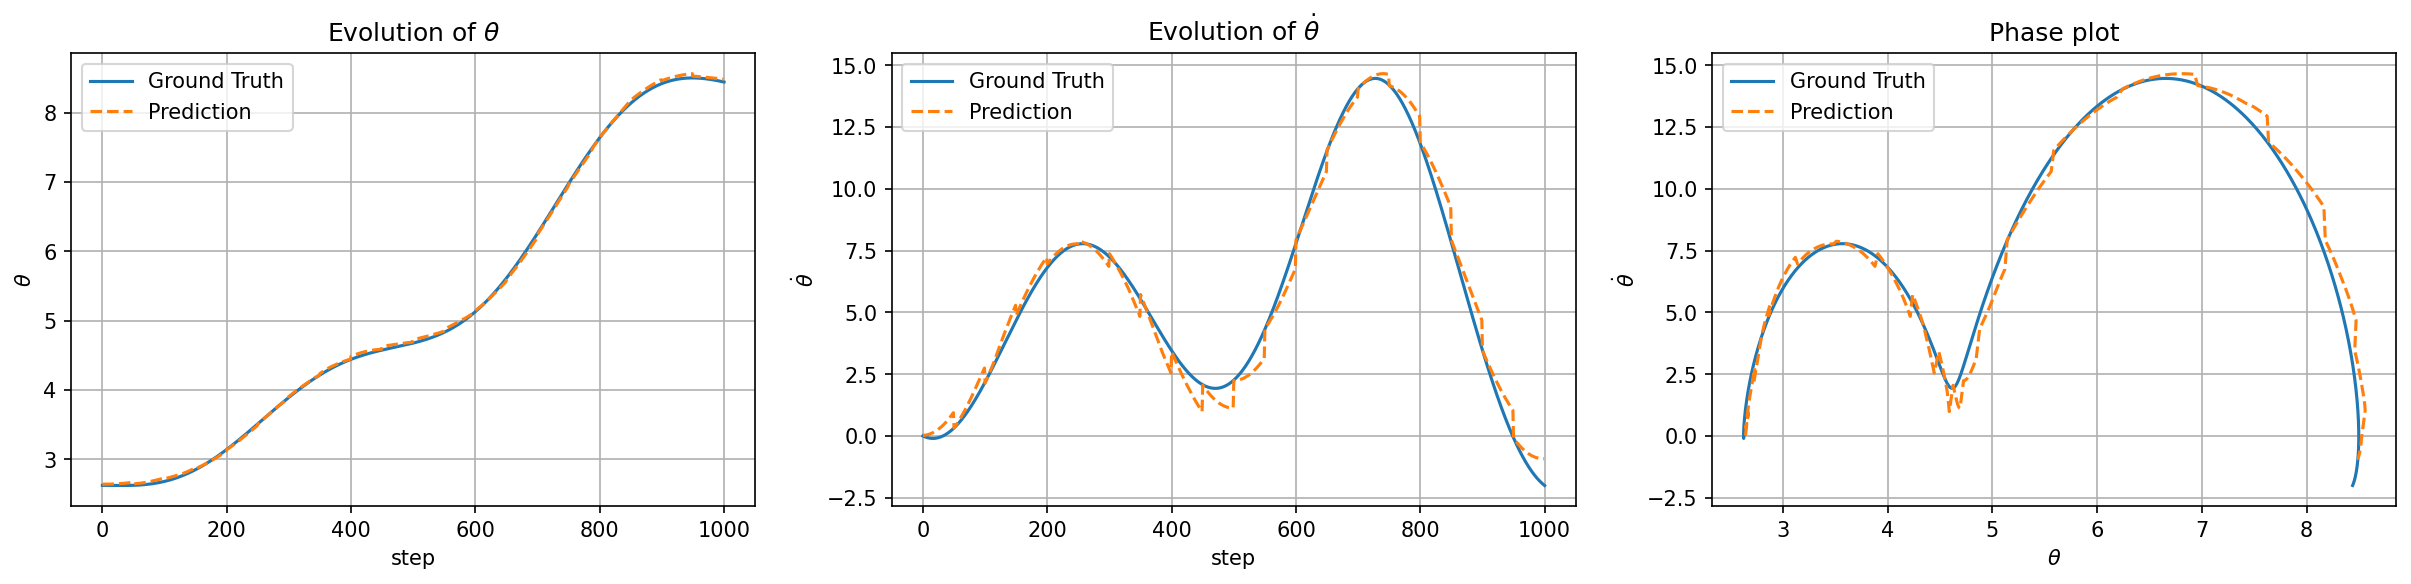
\includegraphics[width=\textwidth]{koopman_correct}
  \caption{Identified Pendulum with Koopman Space Prediction (with periodic correction)}
  \label{fig:koopman_correct}
\end{figure}

\begin{figure}[htb!]
  \centering
  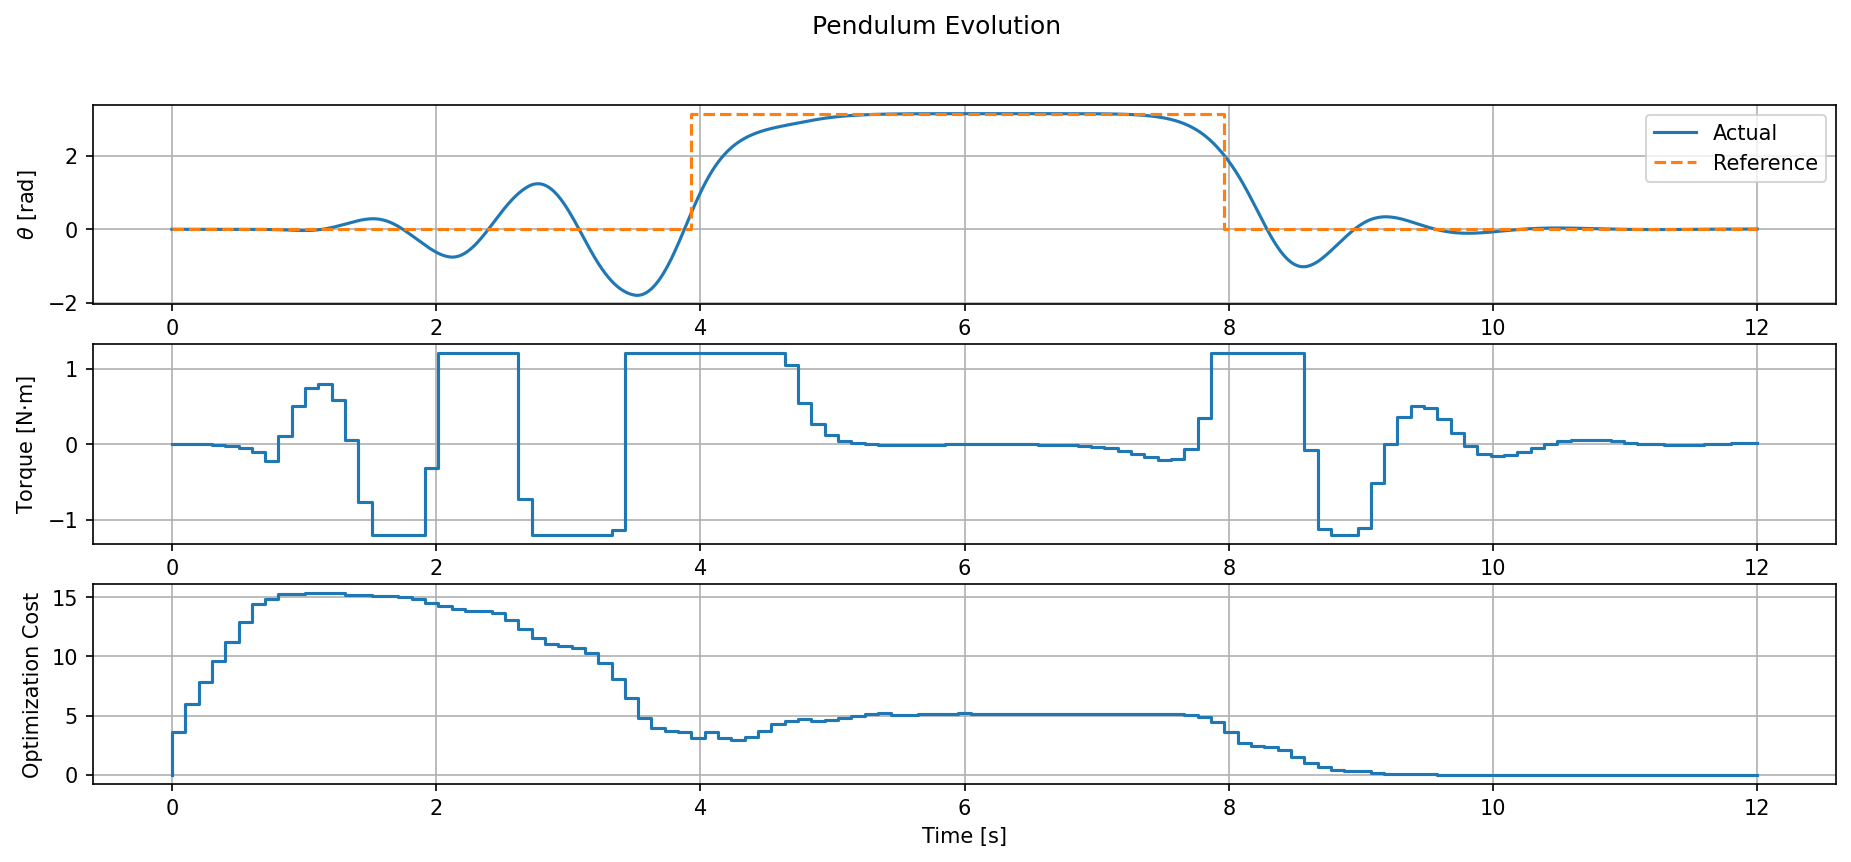
\includegraphics[width=\textwidth]{mpc_pendulum}
  \caption{SINDYc with MPC -- Pendulum Control}
  \label{fig:mpc_pendulum}
\end{figure}

\begin{figure}[htb!]
  \centering
  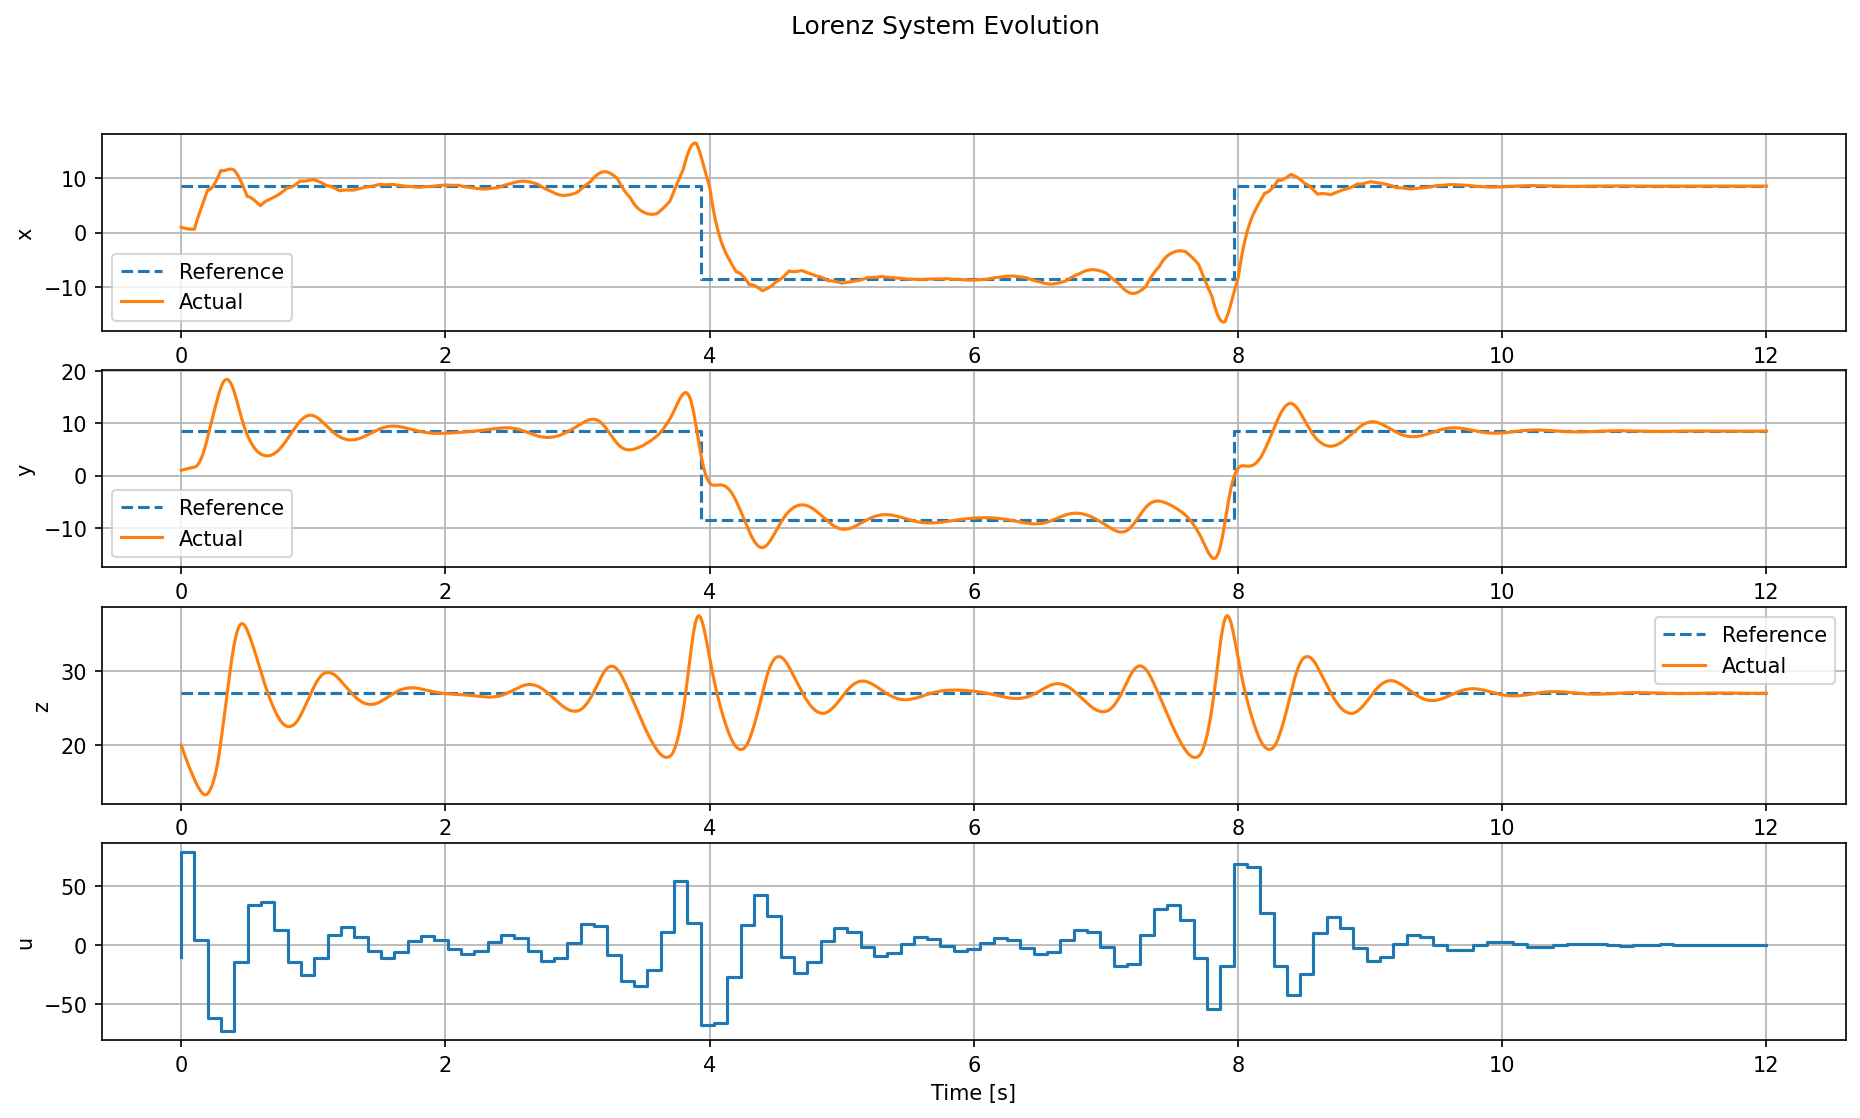
\includegraphics[width=\textwidth]{mpc_lorenz}
  \caption{SINDYc with MPC -- Lorenz Attractor Control}
  \label{fig:mpc_lorenz}
\end{figure}

\begin{figure}[htb!]
  \centering
  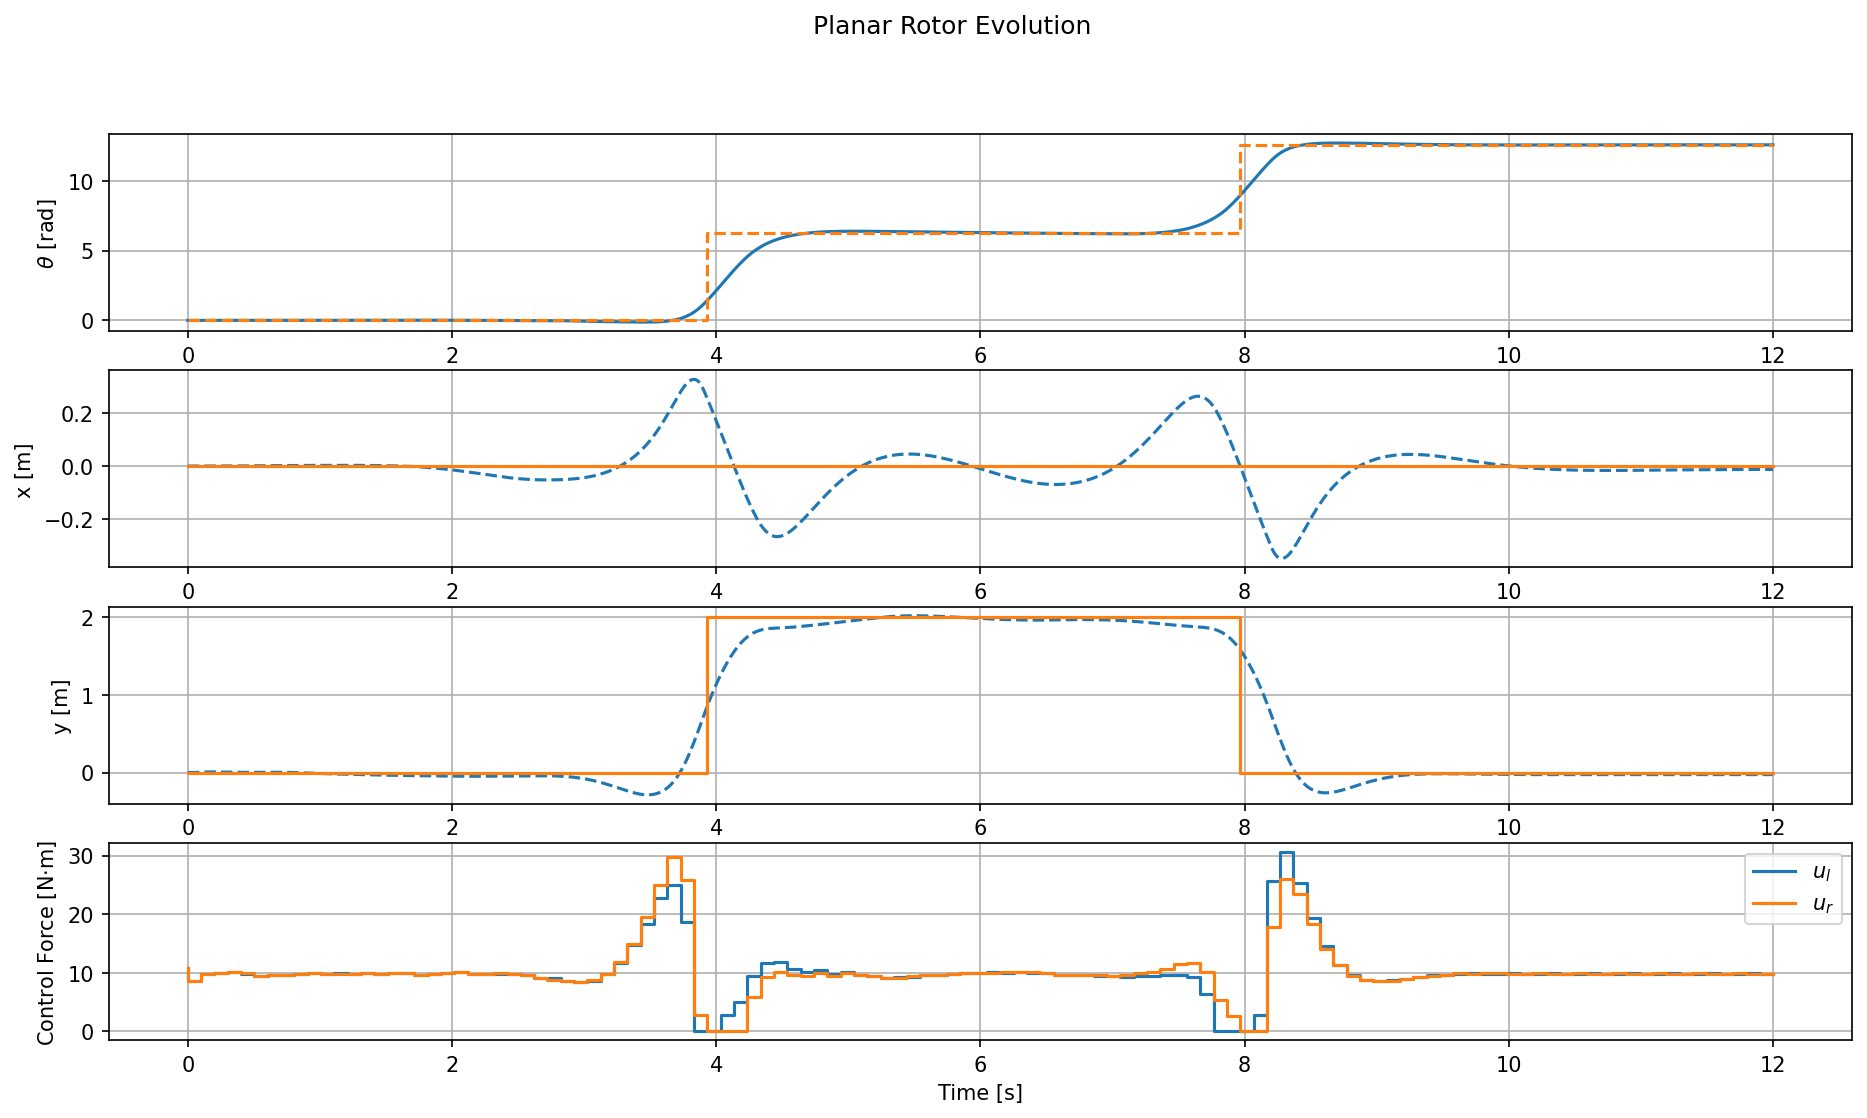
\includegraphics[width=\textwidth]{mpc_rotor}
  \caption{SINDYc with MPC -- Planar Rotor Control}
  \label{fig:mpc_rotor}
\end{figure}

\end{document}
